\documentclass[a4paper]{article}
\usepackage[T1]{fontenc}
\usepackage{amsmath}
\usepackage{amssymb}
\usepackage{xcolor}
\usepackage{tikz}
\usetikzlibrary{arrows,shapes.geometric,positioning,shadows,calc,backgrounds}

\begin{document}

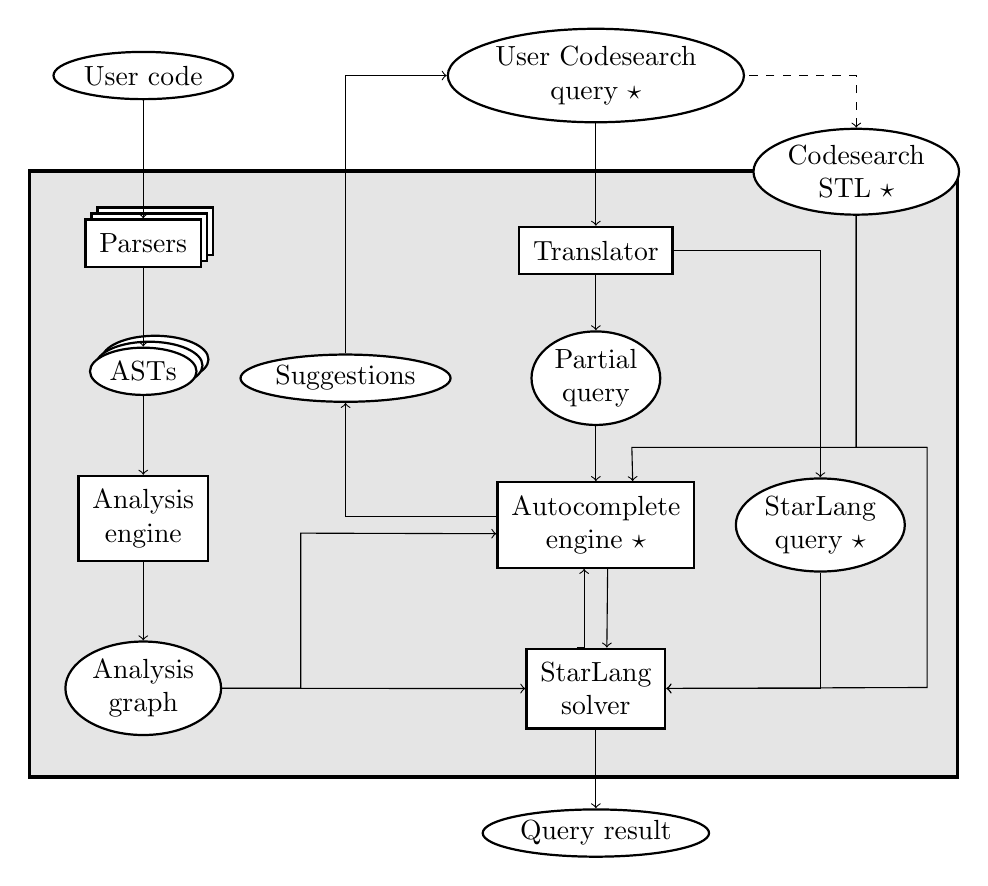
\begin{tikzpicture}[
  every node/.style={inner sep=1.5pt},
  data/.style={ellipse, draw=black, fill=white, thick, minimum height=4mm, minimum height=6mm, align=center},
  process/.style={rectangle, draw=black, fill=white, thick, minimum width=5mm, minimum height=6mm, align=center, inner sep=5pt},
  shadows/.style={double copy shadow, shadow xshift=2pt, shadow yshift=-2pt},
]
  %nodes
  \node[data] (code) {User code};
  \node[data] (query) [right=of code,xshift=1.7cm] {User Codesearch\\query $\star$};
  \node[process, shadows] (parsers) [below=of code,yshift=-0.5cm] {Parsers};
  \node[data, shadows] (asts) [below=of parsers] {ASTs};
  \node[process] (engine) [below=of asts] {Analysis\\engine};
  \node[data] (graph) [below=of engine,yshift=0.1mm] {Analysis\\graph};
  \node[process] (translator) [below=of query,yshift=-0.3cm] {Translator};
  \node[data] (stdlib) [right=of translator,yshift=10mm] {Codesearch\\STL $\star$};
  \node[data] (partial-query) [below=of translator,yshift=0.3cm] {Partial\\query};
  \node[process] (autocomplete) [below=of partial-query,yshift=0.3cm] {Autocomplete\\engine $\star$};
  \node[process] (solver) [below=of autocomplete] {StarLang\\solver};
  \node[data] (starlang-query) [right=of autocomplete,xshift=-5mm] {StarLang\\query $\star$};
  \node[data] (suggestions) [left=of partial-query] {Suggestions};
  \node[data] (result) [below=of solver] {Query result};

  %edges
  \draw[->] (code) -- (parsers);
  \draw[->] (parsers) -- (asts);
  \draw[->] (asts) -- (engine);
  \draw[->] (engine) -- (graph);
  \draw[->] (graph) -- (solver);
  \draw[->] (graph) -| +(2,1.97) -- (autocomplete.185);
  \draw[->] (partial-query) -- (autocomplete);
  \draw[->] (translator) -- (partial-query);
  \draw[->] (query) -- (translator);
  \draw[<-,dashed] (stdlib) |- (query);
  \draw[->] (translator) -| (starlang-query);
  \draw[->] (starlang-query) |- (solver);
  \draw[->] (stdlib) |- +(0.9,-3.5) -- +(0.9,-6.55) -- (solver);
  \draw[->] (stdlib) |- +(0.9,-3.5) -- +(-2.85,-3.5) -- (autocomplete.50);
  \draw[->] (solver) -- (result);
  \draw[->] (solver.115) -| (autocomplete.255);
  \draw[->] (autocomplete.285) -- (solver.75);
  \draw[->] (autocomplete.175) -| (suggestions);
  \draw[->] (suggestions) |- (query);

  \begin{scope}[on background layer]
    \draw[very thick,fill=black!10] ($(parsers.north west)+(-0.7,0.6)$) rectangle ($(solver.south east)+(3.7,-0.6)$);
  \end{scope}
\end{tikzpicture}

\end{document}